\section{Robot Design}

The design of the COACHES robots has been carried out within a study made by
the designer Roberto Tino\footnote{www.robertotino.com}, during a collaboration
with Dept. of Computer, Control and Management Engineering Sapienza University of Rome, Italy.


The designed robot model has been called ALFRED and the main design concept has been developed for the need of deploying a social robot in public environments (such as, shopping malls) with the purpose of assisting people that need for help or
information, guiding them to a certain location, etc.

The main results of the design are reported in the following of this section.


\subsection{Motivation and design goals}

In previous years, robots were mostly used within
factories or non-public spaces and thus their look was not
a crucial aspect. The essential thing for a good robot was
to carry out its programmed job in a precise and
repetitive manner. Its shape was designed mainly for
functionality and the interaction with humans was limited
to technicians instructed on how to use them.
Recently, more and more robotic applications have
moved into public space populated by non-expert users.
Consequently, robot appearance started to evolve to adapt
to the public and domestic environments and forms of
natural interactions with users (e.g., speech) are emerging
thanks also to the developments in the field of artificial
intelligence.

Finally, many studies on social robotics require to design and realize robots that can operate in very close
contact with people and can perform in general social acceptable behaviors. The shape of this kind of robots
has a fundamental role; it has to suggest the interaction and to raise the people curiosity. The appearance has
to be friendly and has not to instill dread.

Following this trend, we have designed and developed a social robot for public environment, as described in
the following of this abstract. The design has followed guidelines and use cases of the COACHES project,
that aims at developing autonomous social robots operating in a shopping mall in Caen, France and
performing short-term interactions with shop-keepers and customers of the mall.
Moreover, given the actual goal of fully producing two of these robots to be deployed in a real shopping
mall, architectural and functional limits derived by limited budget have been carefully considered.
The two robots are under development from Algorithmica S.r.l.\footnote{http://algorithmica.it} company and they are expected to be delivered in Fall 2015.

\subsection{Design concepts}

ALFRED is a social robot designed to operate in public environments populated by many non-expert users.
Its main purpose is to assist people that ask for help or information, need to be guided to a certain
location, as well as to advertise items and goods as provided by shop-keepers.
As being in front of something that looks human but is not human can instill dread to the user, we chose not
to use an anthropomorphic shape for the robot.

However, size and shape of the robot resemble those of a human. In this way we expect the robot to suggest
natural human-like interactions (such as, using speech or gestures). The structure is erect and curved ahead to
have a servile aspect and it is not taller than a human.

One main objective of this design was to create a robust and light robot that can stimulate interactions from
users.
The robotic base guarantees a very smooth and agile motion in indoor environments, sensors and
computational power allows for realizing complex behaviors and multi-modal interactions, while the carbon
structure provides robustness and lightness.
The molded components design is very minimal and it is composed of simple shapes, like spheres or
triangles, the surfaces are smooth and accommodating without corners or sharp edges.

The result of the design is illustrated in the following figures.

\begin{center}
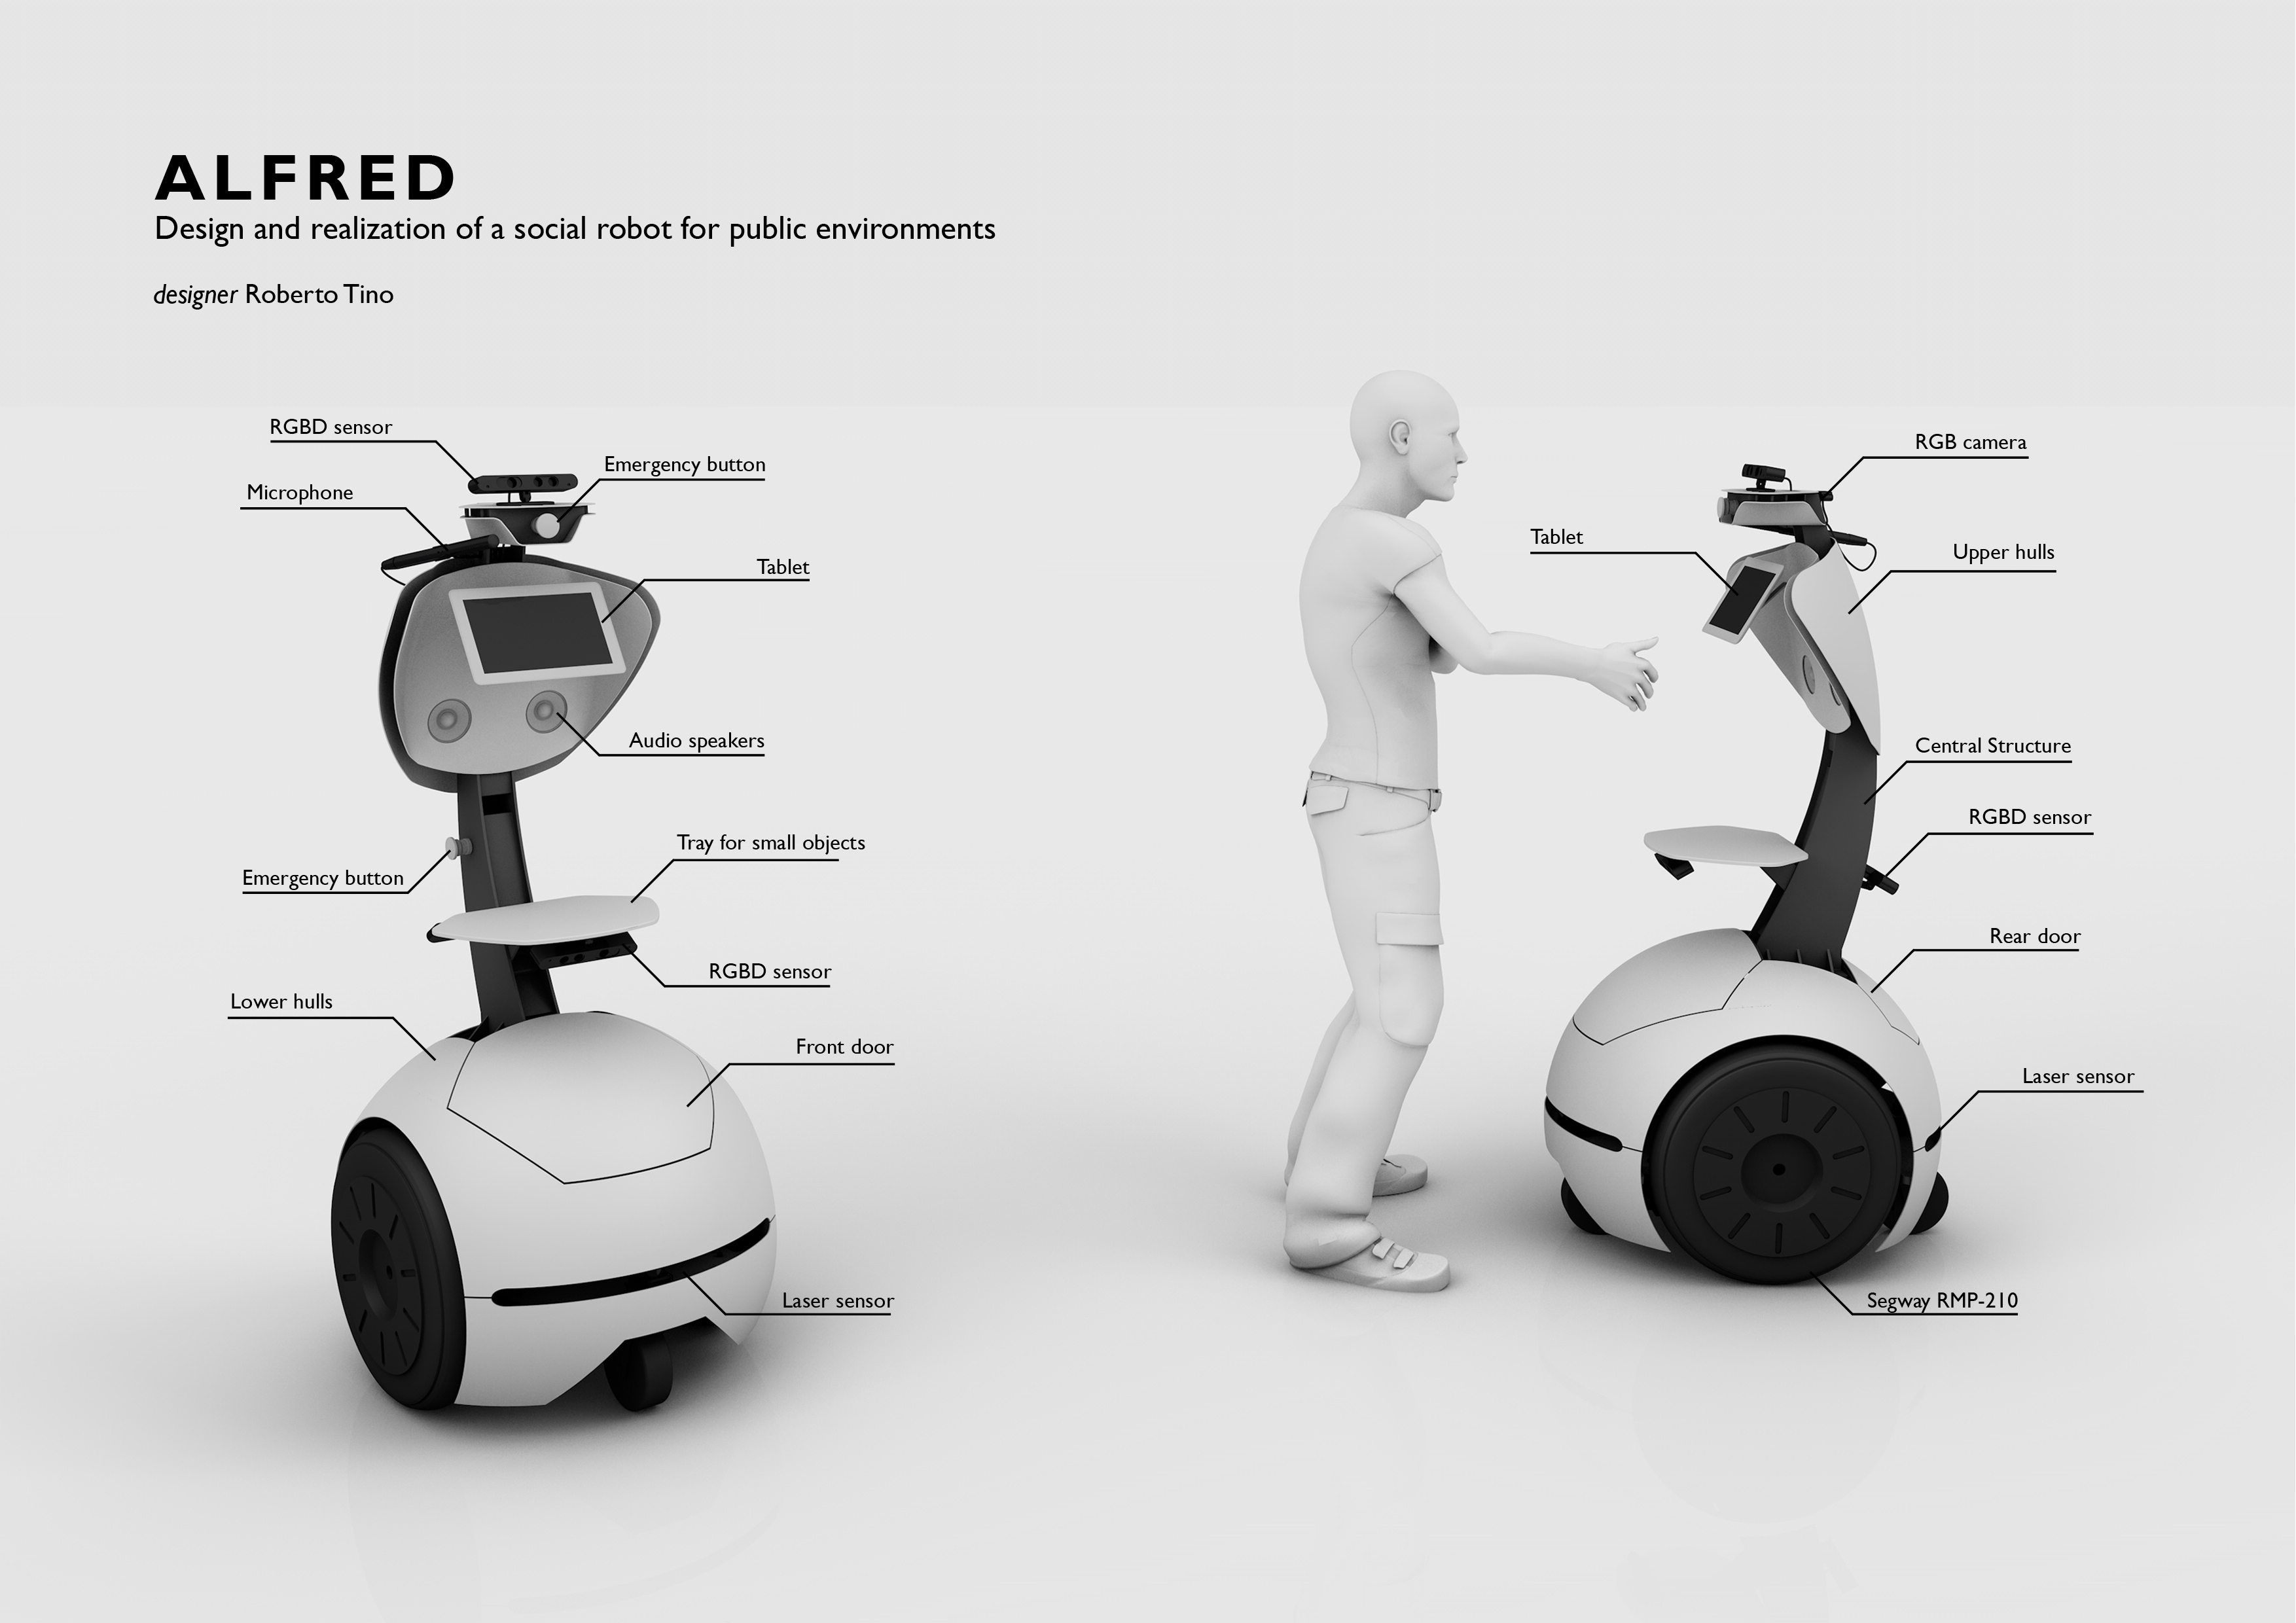
\includegraphics[height=10cm]{fig/Tavola01.jpg}
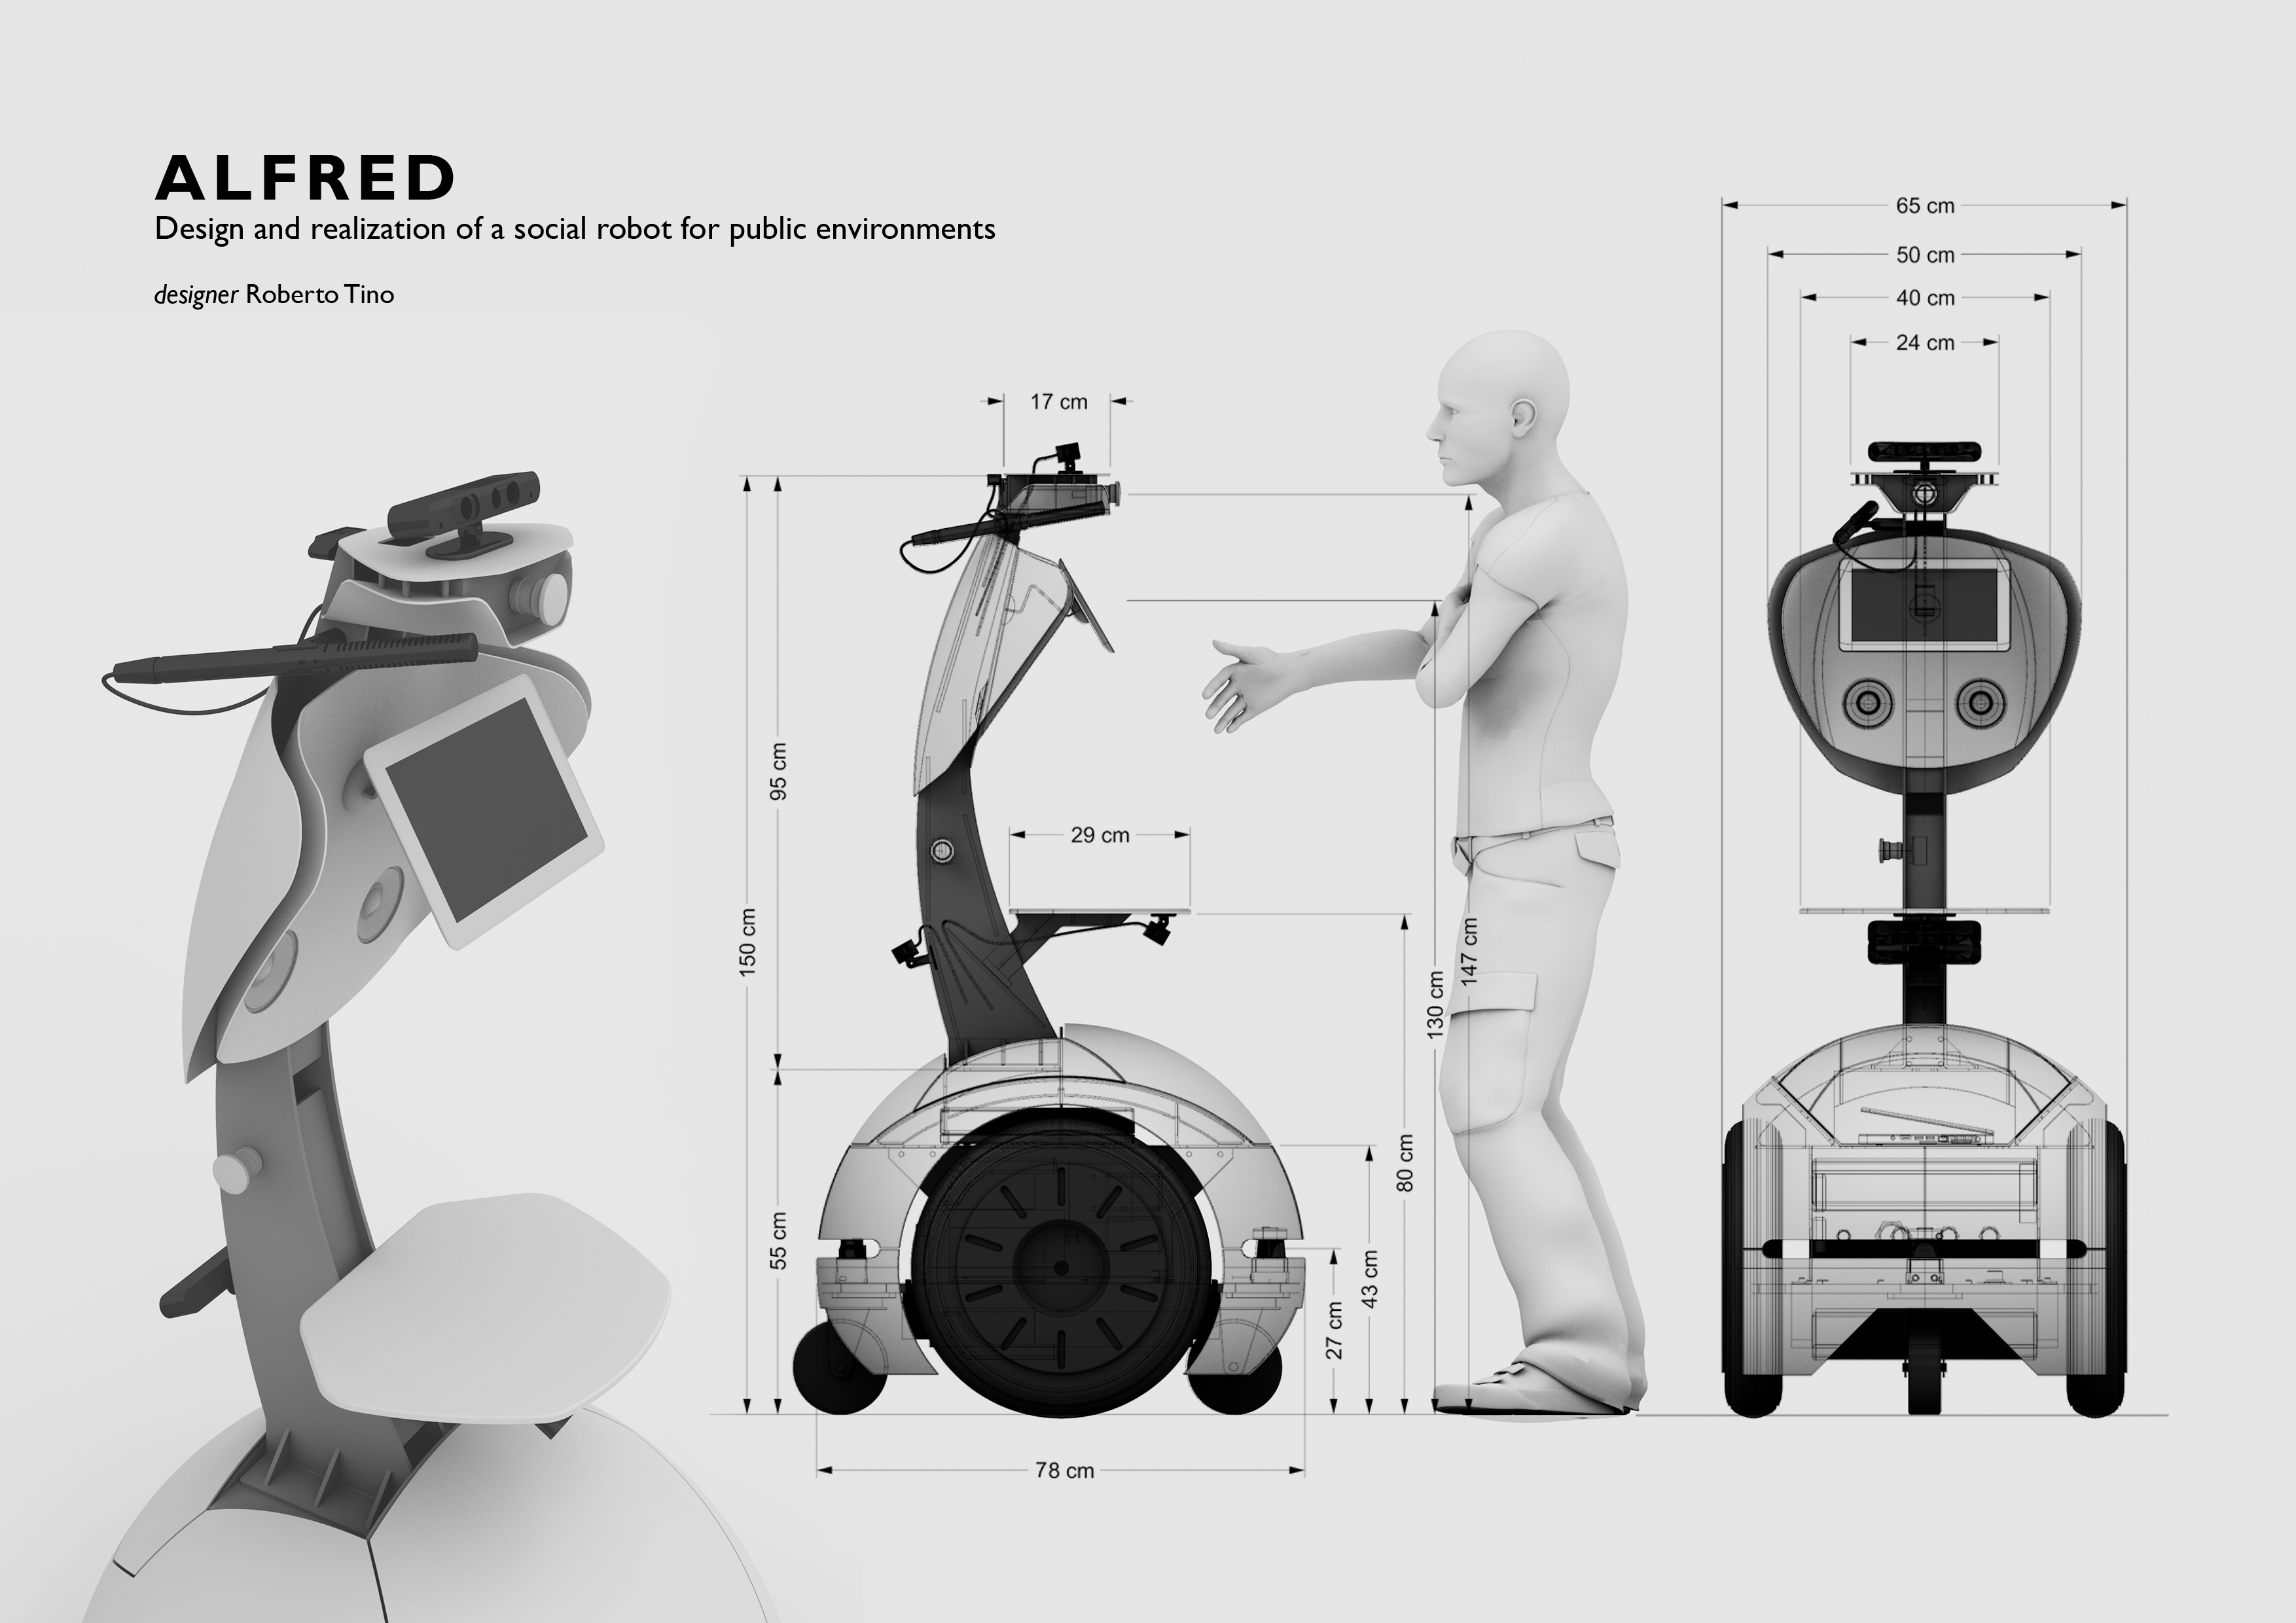
\includegraphics[height=10cm]{fig/Tavola02.jpg}
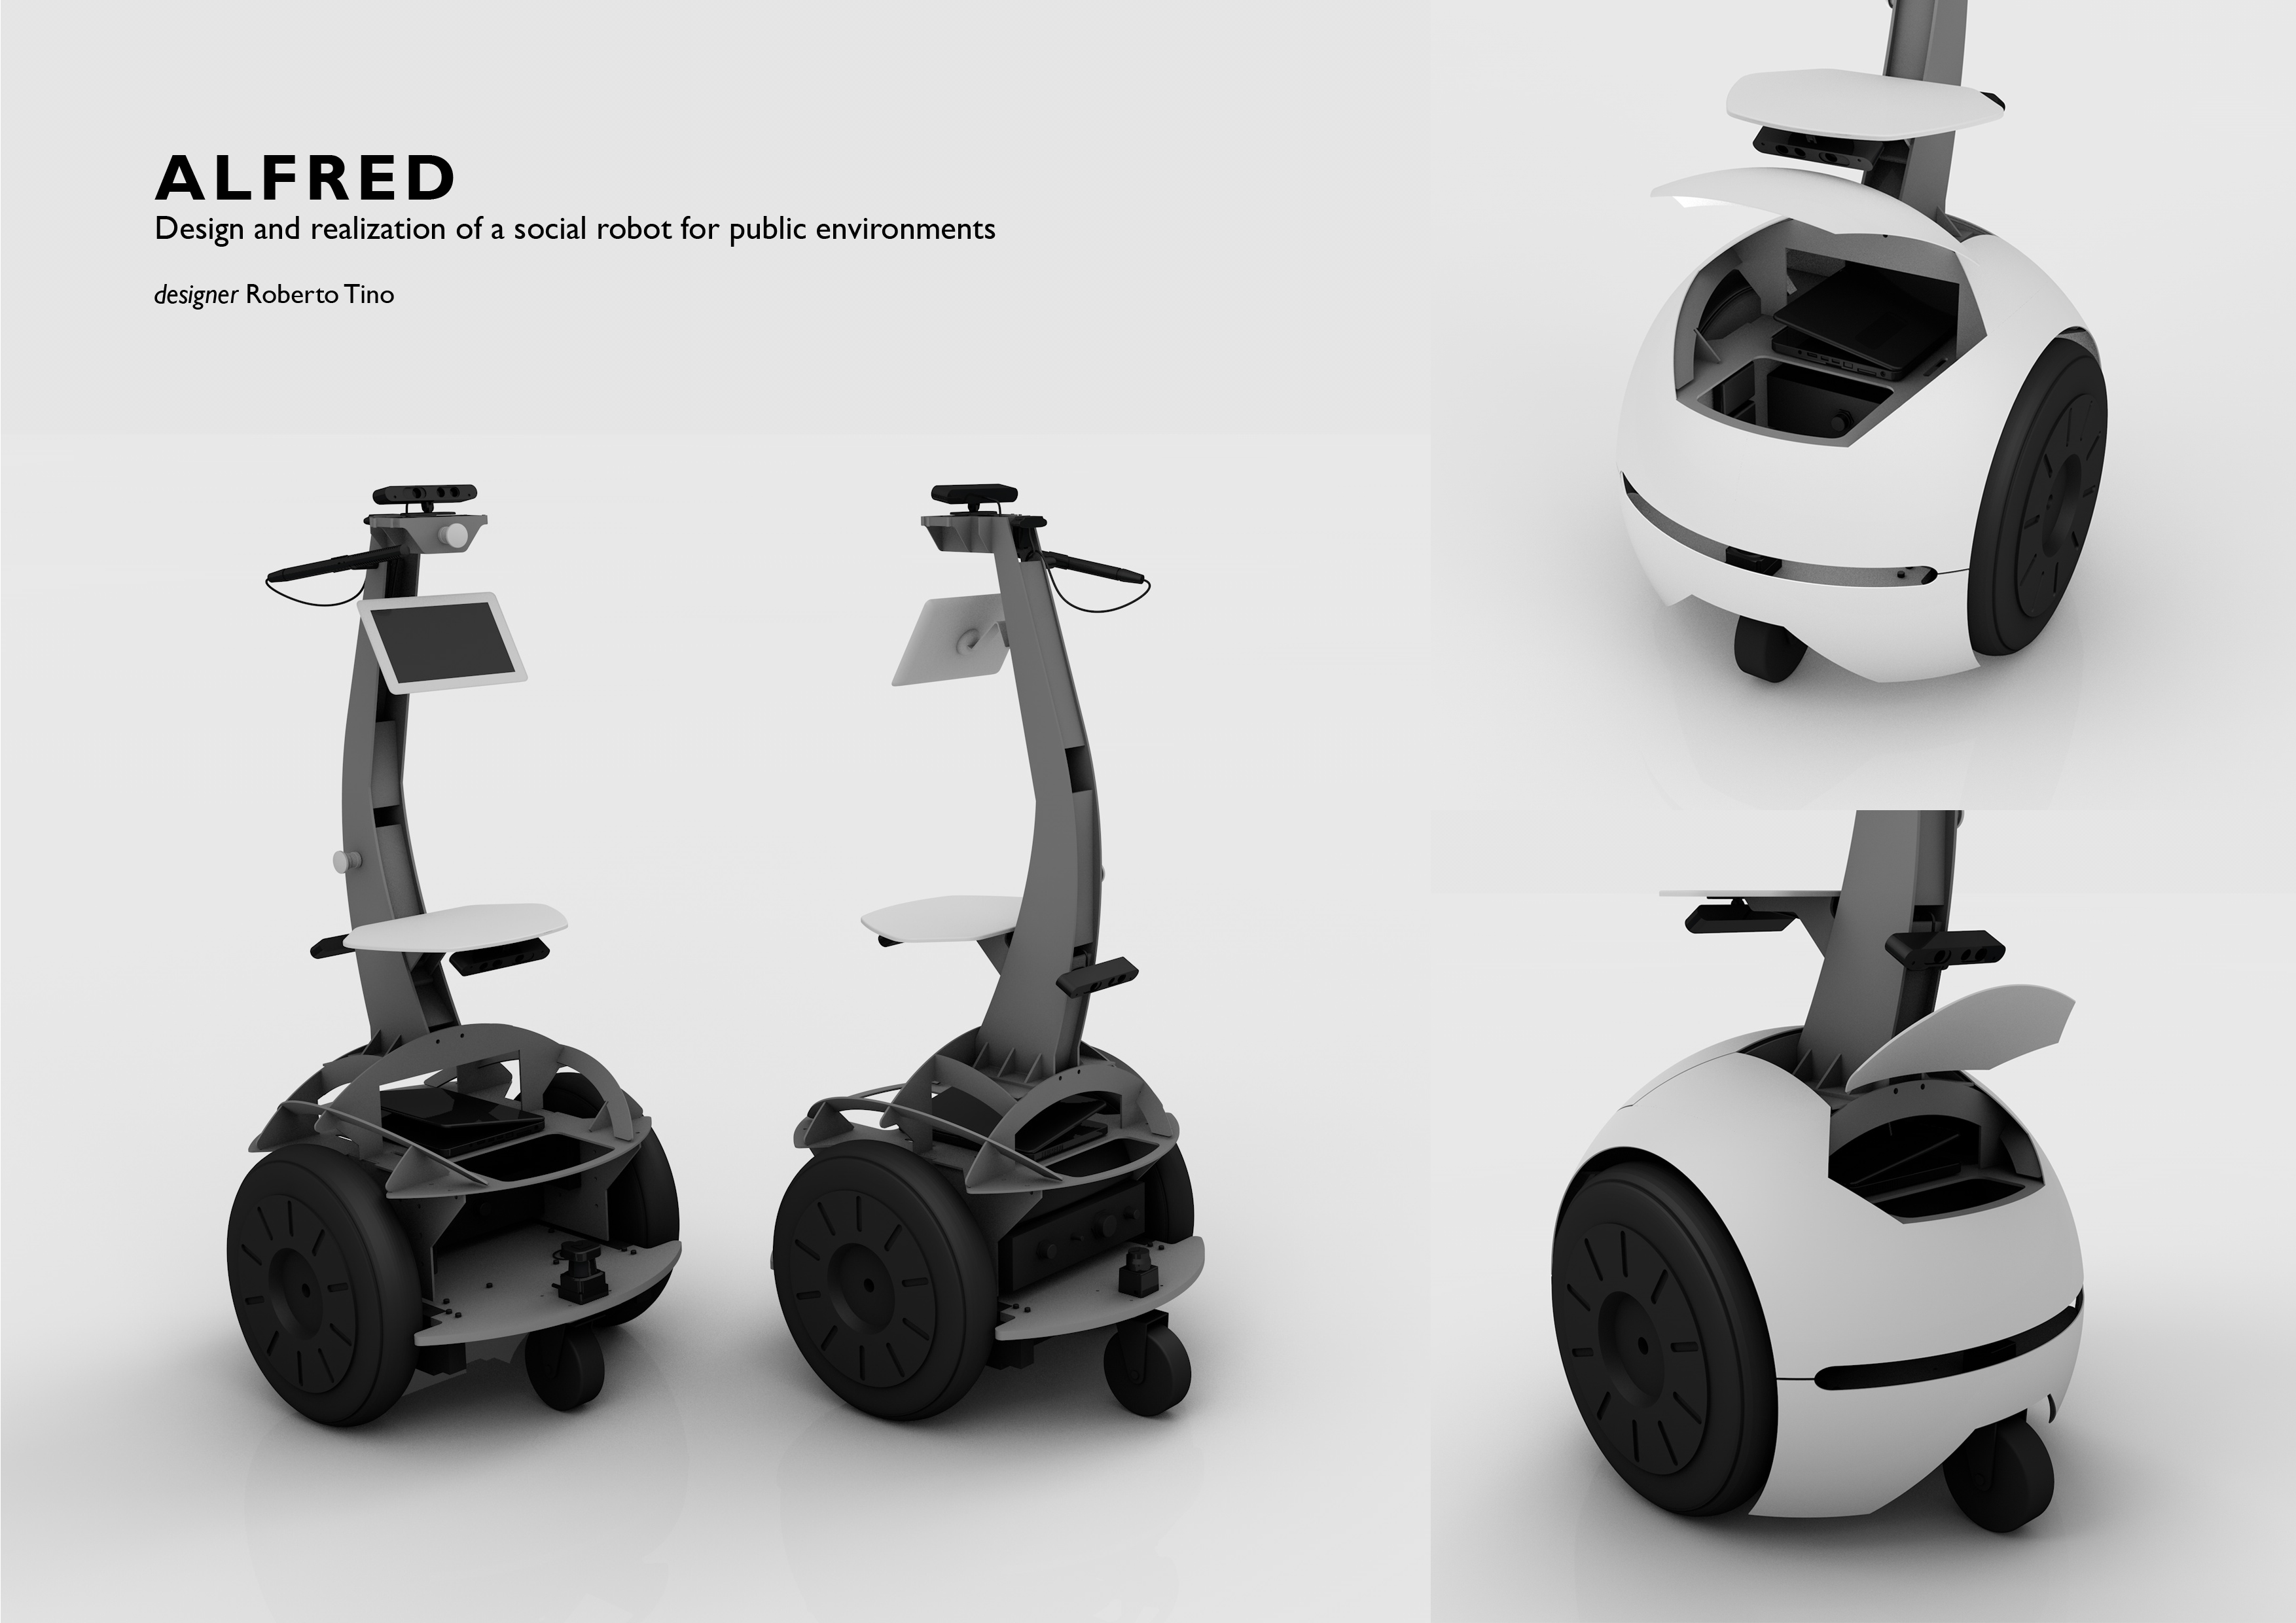
\includegraphics[height=10cm]{fig/Tavola03.jpg}
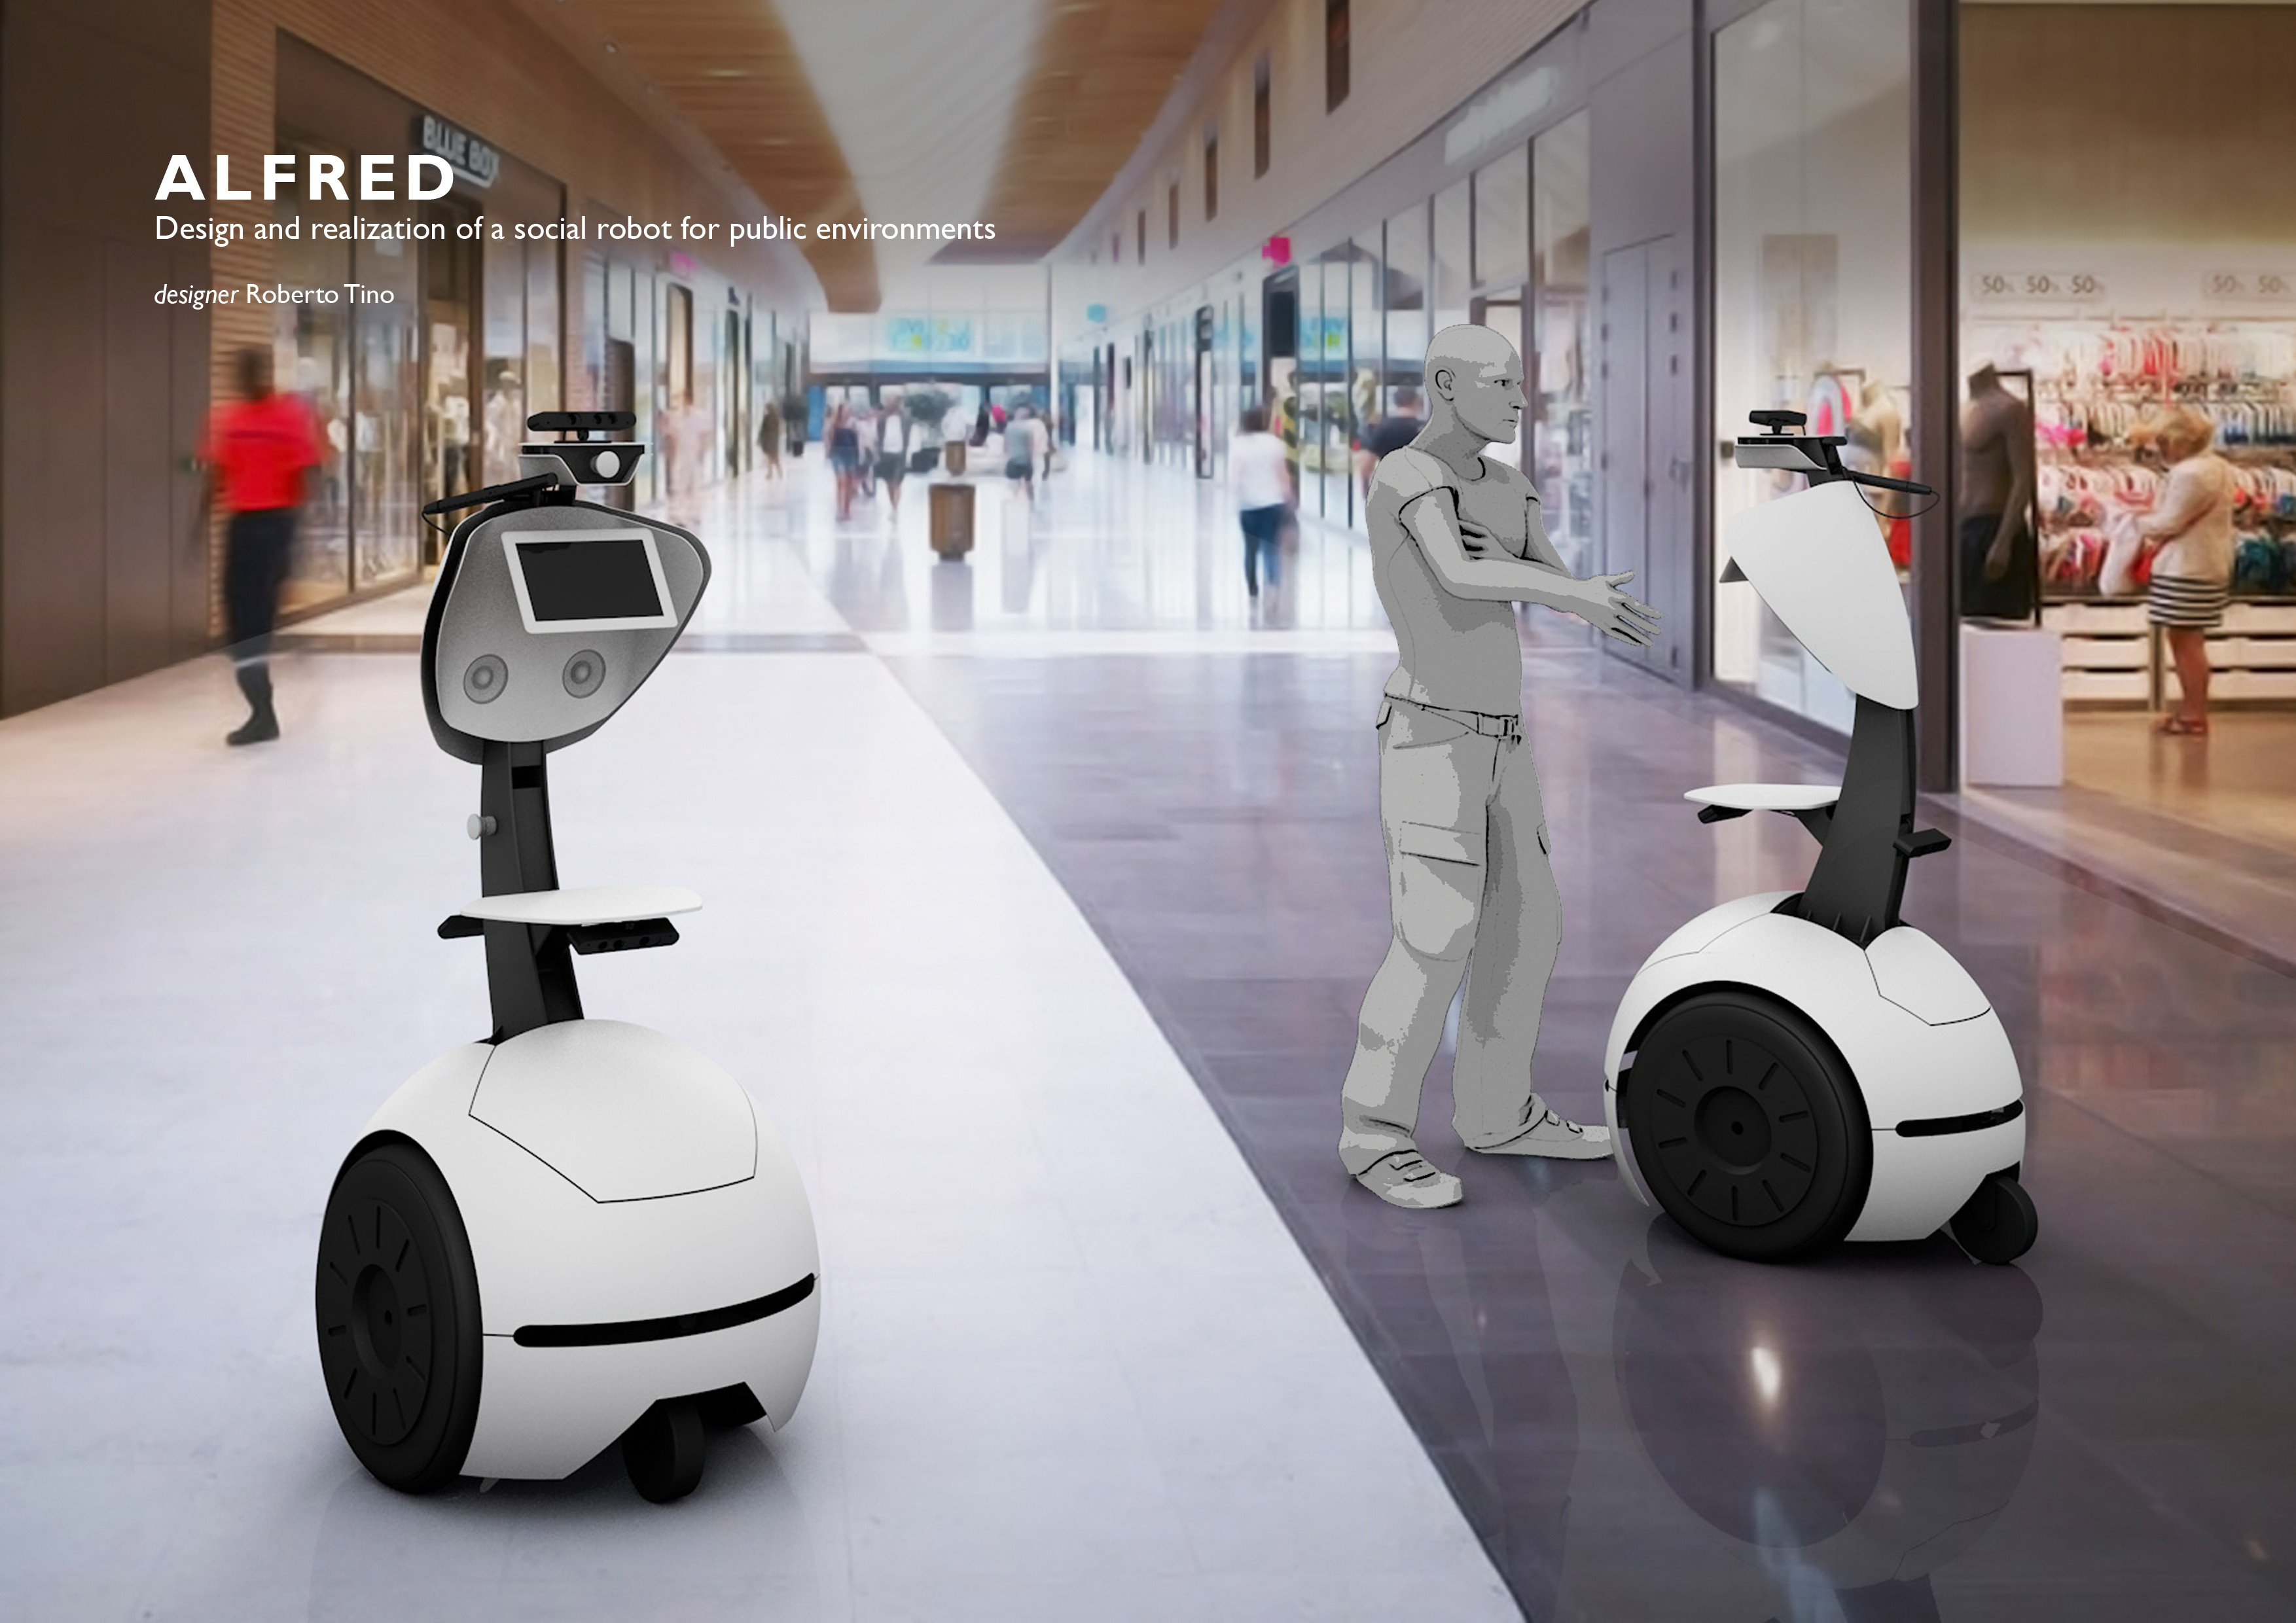
\includegraphics[height=10cm]{fig/Tavola04.jpg}
\end{center}


\subsection{Realization}

The robot is built using a Segway robotic base RMP-210 and it is composed by a central carbon structure
obtained from flat plates that are later dovetailed and glued with each other.
The robot lower casing is designed to host a laptop, two laser sensors and all the electronic needed to control
the robot, while the top partis a sort of backbone that housestwo or three RGBD sensors, a camera, a tablet,
two audio speakers, the microphone and a tray where to place small objects.
External hulls are arranged upon the main structure with the purpose of protecting the components and to
give a pleasant look. The hulls are made of a composite material, laminated on mold previously created.
Finally, the two parts of the robot are easy to disassemblefor transportation.



